

\tikzset{every picture/.style={line width=0.75pt}} %set default line width to 0.75pt        

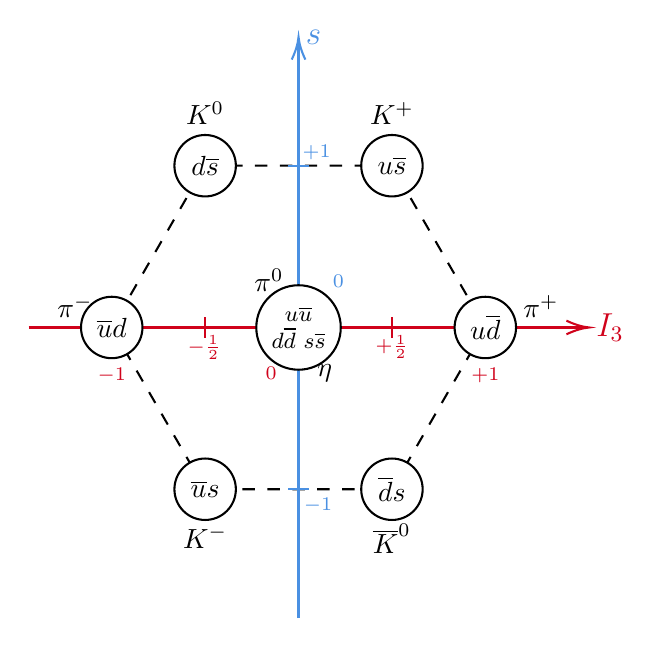
\begin{tikzpicture}[x=0.75pt,y=0.75pt,yscale=-1,xscale=1]
%uncomment if require: \path (0,312); %set diagram left start at 0, and has height of 312

%Shape: Regular Polygon [id:dp00036259320032794307] 
\draw  [dash pattern={on 4.5pt off 4.5pt}] (230,162) -- (185,239.94) -- (95,239.94) -- (50,162) -- (95,84.06) -- (185,84.06) -- cycle ;
%Straight Lines [id:da7432714490785992] 
\draw [color={rgb, 255:red, 208; green, 2; blue, 27 }  ,draw opacity=1 ]   (10,162) -- (278,162) ;
\draw [shift={(280,162)}, rotate = 180] [color={rgb, 255:red, 208; green, 2; blue, 27 }  ,draw opacity=1 ][line width=0.75]    (10.93,-3.29) .. controls (6.95,-1.4) and (3.31,-0.3) .. (0,0) .. controls (3.31,0.3) and (6.95,1.4) .. (10.93,3.29)   ;
%Straight Lines [id:da5800138783290809] 
\draw [color={rgb, 255:red, 74; green, 144; blue, 226 }  ,draw opacity=1 ]   (140,302) -- (140,24) ;
\draw [shift={(140,22)}, rotate = 90] [color={rgb, 255:red, 74; green, 144; blue, 226 }  ,draw opacity=1 ][line width=0.75]    (10.93,-3.29) .. controls (6.95,-1.4) and (3.31,-0.3) .. (0,0) .. controls (3.31,0.3) and (6.95,1.4) .. (10.93,3.29)   ;
%Straight Lines [id:da0424063895802933] 
\draw [color={rgb, 255:red, 208; green, 2; blue, 27 }  ,draw opacity=1 ]   (95,157) -- (95,167) ;
%Straight Lines [id:da5315540321645463] 
\draw [color={rgb, 255:red, 208; green, 2; blue, 27 }  ,draw opacity=1 ]   (185,157) -- (185,167) ;
%Shape: Circle [id:dp9016274878129079] 
\draw  [fill={rgb, 255:red, 255; green, 255; blue, 255 }  ,fill opacity=1 ] (80.2,84.06) .. controls (80.2,75.88) and (86.83,69.26) .. (95,69.26) .. controls (103.17,69.26) and (109.8,75.88) .. (109.8,84.06) .. controls (109.8,92.23) and (103.17,98.86) .. (95,98.86) .. controls (86.83,98.86) and (80.2,92.23) .. (80.2,84.06) -- cycle ;
%Shape: Circle [id:dp26967635701794923] 
\draw  [fill={rgb, 255:red, 255; green, 255; blue, 255 }  ,fill opacity=1 ] (170.2,84.06) .. controls (170.2,75.88) and (176.83,69.26) .. (185,69.26) .. controls (193.17,69.26) and (199.8,75.88) .. (199.8,84.06) .. controls (199.8,92.23) and (193.17,98.86) .. (185,98.86) .. controls (176.83,98.86) and (170.2,92.23) .. (170.2,84.06) -- cycle ;
%Shape: Circle [id:dp829825410707284] 
\draw  [fill={rgb, 255:red, 255; green, 255; blue, 255 }  ,fill opacity=1 ] (35.2,162) .. controls (35.2,153.83) and (41.83,147.2) .. (50,147.2) .. controls (58.17,147.2) and (64.8,153.83) .. (64.8,162) .. controls (64.8,170.17) and (58.17,176.8) .. (50,176.8) .. controls (41.83,176.8) and (35.2,170.17) .. (35.2,162) -- cycle ;
%Shape: Circle [id:dp7821465181120492] 
\draw  [fill={rgb, 255:red, 255; green, 255; blue, 255 }  ,fill opacity=1 ] (215.2,162) .. controls (215.2,153.83) and (221.83,147.2) .. (230,147.2) .. controls (238.17,147.2) and (244.8,153.83) .. (244.8,162) .. controls (244.8,170.17) and (238.17,176.8) .. (230,176.8) .. controls (221.83,176.8) and (215.2,170.17) .. (215.2,162) -- cycle ;
%Shape: Circle [id:dp050740490078981626] 
\draw  [fill={rgb, 255:red, 255; green, 255; blue, 255 }  ,fill opacity=1 ] (80.2,239.94) .. controls (80.2,231.77) and (86.83,225.14) .. (95,225.14) .. controls (103.17,225.14) and (109.8,231.77) .. (109.8,239.94) .. controls (109.8,248.12) and (103.17,254.74) .. (95,254.74) .. controls (86.83,254.74) and (80.2,248.12) .. (80.2,239.94) -- cycle ;
%Shape: Circle [id:dp8501124972426272] 
\draw  [fill={rgb, 255:red, 255; green, 255; blue, 255 }  ,fill opacity=1 ] (170.2,239.94) .. controls (170.2,231.77) and (176.83,225.14) .. (185,225.14) .. controls (193.17,225.14) and (199.8,231.77) .. (199.8,239.94) .. controls (199.8,248.12) and (193.17,254.74) .. (185,254.74) .. controls (176.83,254.74) and (170.2,248.12) .. (170.2,239.94) -- cycle ;
%Shape: Circle [id:dp12490437005601918] 
\draw  [fill={rgb, 255:red, 255; green, 255; blue, 255 }  ,fill opacity=1 ] (119.65,162) .. controls (119.65,150.76) and (128.76,141.65) .. (140,141.65) .. controls (151.24,141.65) and (160.35,150.76) .. (160.35,162) .. controls (160.35,173.24) and (151.24,182.35) .. (140,182.35) .. controls (128.76,182.35) and (119.65,173.24) .. (119.65,162) -- cycle ;
%Straight Lines [id:da10691295631235598] 
\draw [color={rgb, 255:red, 74; green, 144; blue, 226 }  ,draw opacity=1 ]   (135,84.06) -- (145,84.06) ;
%Straight Lines [id:da40035051048673465] 
\draw [color={rgb, 255:red, 74; green, 144; blue, 226 }  ,draw opacity=1 ]   (135,239.9) -- (145,239.9) ;

% Text Node
\draw (142,22) node [anchor=west] [inner sep=0.75pt]  [font=\large,color={rgb, 255:red, 74; green, 144; blue, 226 }  ,opacity=1 ]  {$s$};
% Text Node
\draw (282,162) node [anchor=west] [inner sep=0.75pt]  [font=\large,color={rgb, 255:red, 208; green, 2; blue, 27 }  ,opacity=1 ]  {$I_{3}$};
% Text Node
\draw (140.5,72.65) node [anchor=north west][inner sep=0.75pt]  [font=\fontsize{0.71em}{0.85em}\selectfont,color={rgb, 255:red, 74; green, 144; blue, 226 }  ,opacity=1 ]  {$+1$};
% Text Node
\draw (141.08,242.57) node [anchor=north west][inner sep=0.75pt]  [font=\fontsize{0.71em}{0.85em}\selectfont,color={rgb, 255:red, 74; green, 144; blue, 226 }  ,opacity=1 ]  {$-1$};
% Text Node
\draw (50,180.2) node [anchor=north] [inner sep=0.75pt]  [font=\fontsize{0.71em}{0.85em}\selectfont,color={rgb, 255:red, 208; green, 2; blue, 27 }  ,opacity=1 ]  {$-1$};
% Text Node
\draw (230,180.2) node [anchor=north] [inner sep=0.75pt]  [font=\fontsize{0.71em}{0.85em}\selectfont,color={rgb, 255:red, 208; green, 2; blue, 27 }  ,opacity=1 ]  {$+1$};
% Text Node
\draw (185.09,164.28) node [anchor=north] [inner sep=0.75pt]  [font=\fontsize{0.71em}{0.85em}\selectfont,color={rgb, 255:red, 208; green, 2; blue, 27 }  ,opacity=1 ]  {$+\frac{1}{2}$};
% Text Node
\draw (94.65,164.6) node [anchor=north] [inner sep=0.75pt]  [font=\fontsize{0.71em}{0.85em}\selectfont,color={rgb, 255:red, 208; green, 2; blue, 27 }  ,opacity=1 ]  {$-\frac{1}{2}$};
% Text Node
\draw (95,84.06) node    {$d\overline{s}$};
% Text Node
\draw (185,84.06) node    {$u\overline{s}$};
% Text Node
\draw (50,162) node    {$\overline{u} d$};
% Text Node
\draw (230,162) node    {$u\overline{d}$};
% Text Node
\draw (95,239.94) node    {$\overline{u} s$};
% Text Node
\draw (185,239.94) node    {$\overline{d} s$};
% Text Node
\draw (95,65.86) node [anchor=south] [inner sep=0.75pt]    {$K^{0}$};
% Text Node
\draw (185,65.86) node [anchor=south] [inner sep=0.75pt]    {$K^{+}$};
% Text Node
\draw (95,256.14) node [anchor=north] [inner sep=0.75pt]    {$K^{-}$};
% Text Node
\draw (185,255.14) node [anchor=north] [inner sep=0.75pt]    {$\overline{K}^{0}$};
% Text Node
\draw (42.38,158.82) node [anchor=south east] [inner sep=0.75pt]    {$\pi ^{-}$};
% Text Node
\draw (246.8,158.6) node [anchor=south west] [inner sep=0.75pt]    {$\pi ^{+}$};
% Text Node
\draw (134.27,146.09) node [anchor=south east] [inner sep=0.75pt]    {$\pi ^{0}$};
% Text Node
\draw (147.6,178.55) node [anchor=north west][inner sep=0.75pt]    {$\eta $};
% Text Node
\draw (140,162) node  [font=\fontsize{0.8em}{0.96em}\selectfont] [align=left] {\begin{minipage}[lt]{24.07pt}\setlength\topsep{0pt}
\begin{center}
$\displaystyle u\overline{u}$\\$\displaystyle d\overline{d}$ $\displaystyle s\overline{s}$
\end{center}

\end{minipage}};
% Text Node
\draw (131,179.4) node [anchor=north east] [inner sep=0.75pt]  [font=\fontsize{0.71em}{0.85em}\selectfont,color={rgb, 255:red, 208; green, 2; blue, 27 }  ,opacity=1 ]  {$0$};
% Text Node
\draw (155,135.4) node [anchor=north west][inner sep=0.75pt]  [font=\fontsize{0.71em}{0.85em}\selectfont,color={rgb, 255:red, 74; green, 144; blue, 226 }  ,opacity=1 ]  {$0$};


\end{tikzpicture}
